\documentclass[11pt,a4paper]{report}
\usepackage[textwidth=37em,vmargin=30mm]{geometry}
\usepackage{calc,xunicode,amsmath,amssymb,paralist,enumitem,tabu,booktabs,datetime2,xeCJK,xeCJKfntef,listings}
\usepackage{tocloft,fancyhdr,tcolorbox,xcolor,graphicx,eso-pic,xltxtra,xelatexemoji}

\newcommand{\envyear}[0]{2025}
\newcommand{\envdatestr}[0]{2025-03-07}
\newcommand{\envfinaldir}[0]{webdb/2025/20250307/final}

\usepackage[hidelinks]{hyperref}
\hypersetup{
    colorlinks=false,
    pdfpagemode=FullScreen,
    pdftitle={Web Digest - \envdatestr}
}

\setlength{\cftbeforechapskip}{10pt}
\renewcommand{\cftchapfont}{\rmfamily\bfseries\large\raggedright}
\setlength{\cftbeforesecskip}{2pt}
\renewcommand{\cftsecfont}{\sffamily\small\raggedright}

\setdefaultleftmargin{2em}{2em}{1em}{1em}{1em}{1em}

\usepackage{xeCJK,xeCJKfntef}
\xeCJKsetup{PunctStyle=plain,RubberPunctSkip=false,CJKglue=\strut\hskip 0pt plus 0.1em minus 0.05em,CJKecglue=\strut\hskip 0.22em plus 0.2em}
\XeTeXlinebreaklocale "zh"
\XeTeXlinebreakskip = 0pt


\setmainfont{Brygada 1918}
\setromanfont{Brygada 1918}
\setsansfont{IBM Plex Sans}
\setmonofont{JetBrains Mono NL}
\setCJKmainfont{Noto Serif CJK SC}
\setCJKromanfont{Noto Serif CJK SC}
\setCJKsansfont{Noto Sans CJK SC}
\setCJKmonofont{Noto Sans CJK SC}

\setlength{\parindent}{0pt}
\setlength{\parskip}{8pt}
\linespread{1.15}

\lstset{
	basicstyle=\ttfamily\footnotesize,
	numbersep=5pt,
	backgroundcolor=\color{black!5},
	showspaces=false,
	showstringspaces=false,
	showtabs=false,
	tabsize=2,
	captionpos=b,
	breaklines=true,
	breakatwhitespace=true,
	breakautoindent=true,
	linewidth=\textwidth
}






\newcommand{\coverpic}[2]{
    % argv: itemurl, authorname
    Cover photo by #2~~(\href{#1}{#1})
}
\newcommand{\makeheader}[0]{
    \begin{titlepage}
        % \newgeometry{hmargin=15mm,tmargin=21mm,bmargin=12mm}
        \begin{center}
            
            \rmfamily\scshape
            \fontspec{BaskervilleF}
            \fontspec{Old Standard}
            \fontsize{59pt}{70pt}\selectfont
            WEB\hfill DIGEST
            
            \vfill
            % \vskip 30pt
            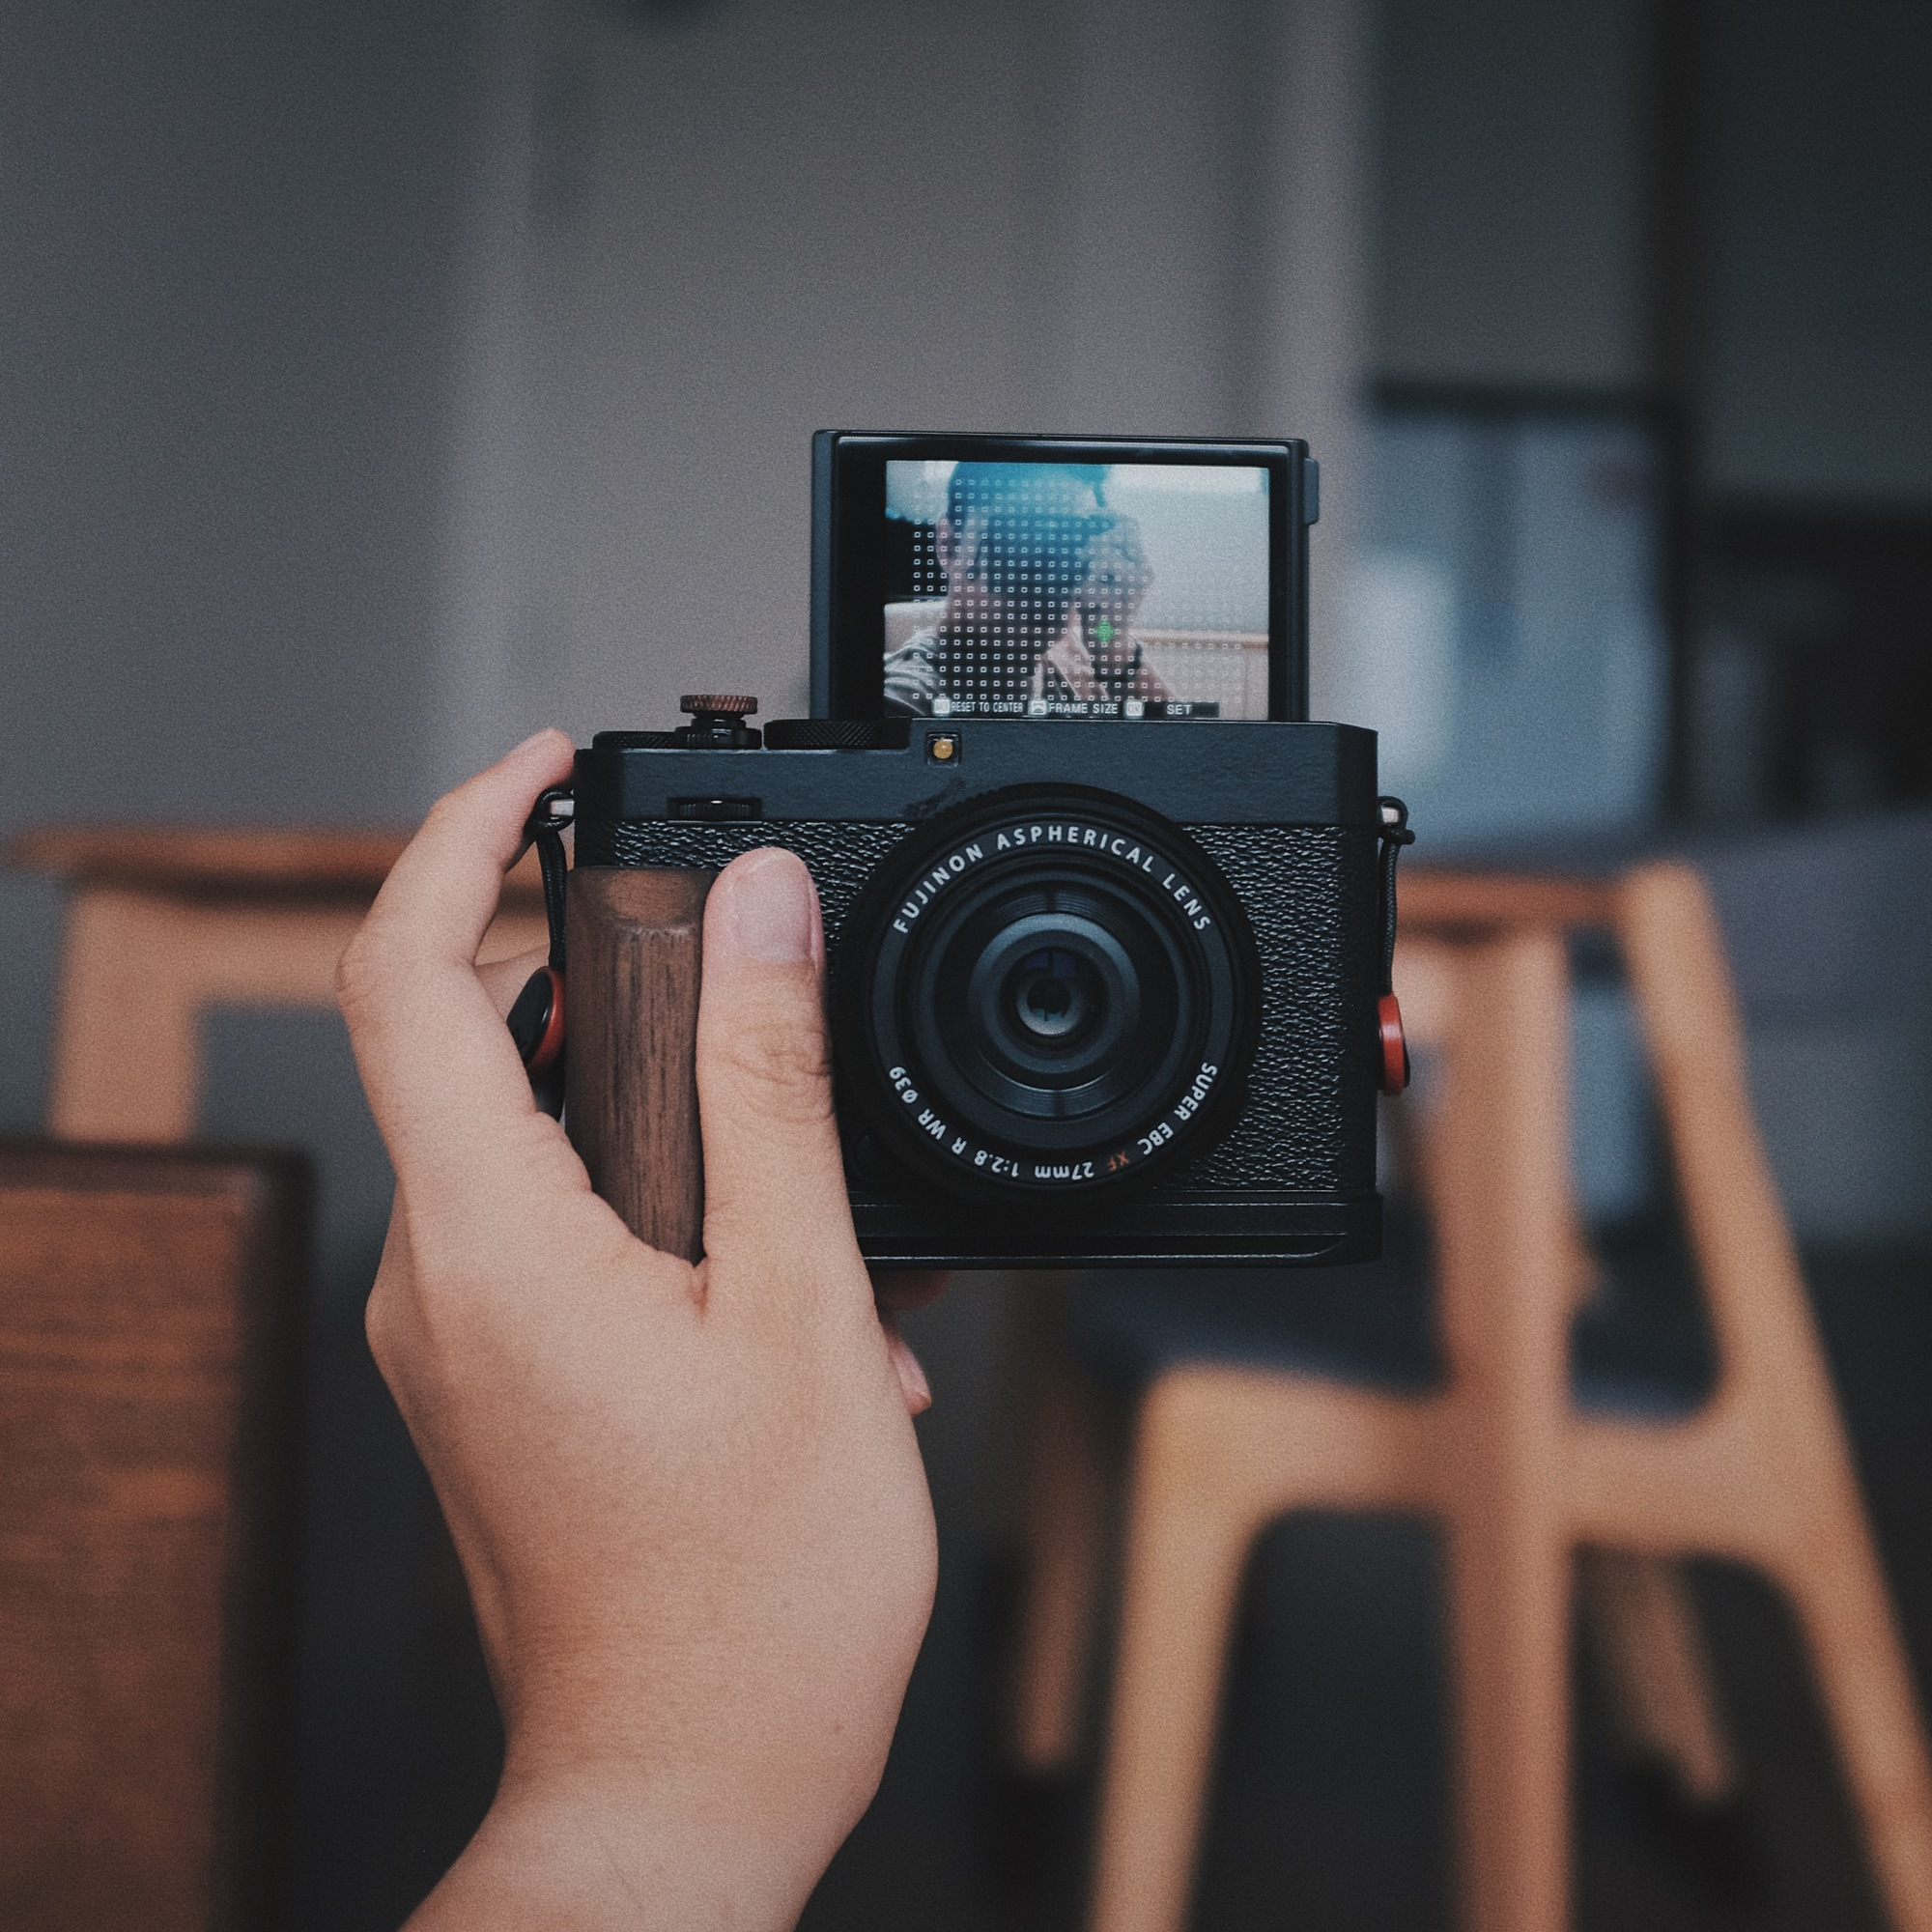
\includegraphics[width=\linewidth]{\envfinaldir/coverpic-prod.jpg}\par
            % \vskip 30pt
            \vfill

            \normalsize\rmfamily\scshape
            \copyright{} The Web Digest Project \hfill\large \envdatestr
        \end{center}
    \end{titlepage}
    % \restoregeometry
}
\newcommand{\simplehref}[1]{%
    \textcolor{blue!80!green}{\href{#1}{#1}}%
}
\renewcommand{\contentsname}{\center\Huge\sffamily\bfseries Contents\par\vskip 20pt}
\newcounter{ipartcounter}
\setcounter{ipartcounter}{0}
\newcommand{\ipart}[1]{
    % \vskip 20pt
    \clearpage
    \stepcounter{ipartcounter}
    \phantomsection
    \addcontentsline{toc}{chapter}{#1}
    % \begin{center}
    %     \Huge
    %     \sffamily\bfseries
    %     #1
    % \end{center}
    % \vskip 20pt plus 7pt
}
\newcounter{ichaptercounter}
\setcounter{ichaptercounter}{0}
\newcommand{\ichapter}[1]{
    % \vskip 20pt
    \clearpage
    \stepcounter{ichaptercounter}
    \phantomsection
    \addcontentsline{toc}{section}{\numberline{\arabic{ichaptercounter}}#1}
    \begin{center}
        \Huge
        \sffamily\bfseries
        #1
    \end{center}
    \vskip 20pt plus 7pt
}
\newcommand{\entrytitlefont}[1]{\subsection*{\raggedright\Large\sffamily\bfseries#1}}
\newcommand{\entryitemGeneric}[2]{
    % argv: title, url
    \parbox{\linewidth}{
        \entrytitlefont{#1}\par\vskip 5pt
        \footnotesize\ttfamily\mdseries
        \simplehref{#2}
    }\vskip 11pt plus 11pt minus 1pt
}
\newcommand{\entryitemGithub}[3]{
    % argv: title, url, desc
    \parbox{\linewidth}{
        \entrytitlefont{#1}\par\vskip 5pt
        \footnotesize\ttfamily\mdseries
        \simplehref{#2}\par\vskip 5pt
        \small\rmfamily\mdseries#3
    }\vskip 11pt plus 11pt minus 1pt
}
\newcommand{\entryitemAp}[3]{
    % argv: title, url, desc
    \parbox{\linewidth}{
        \entrytitlefont{#1}\par\vskip 5pt
        \footnotesize\ttfamily\mdseries
        \simplehref{#2}\par\vskip 5pt
        \small\rmfamily\mdseries#3
    }\vskip 11pt plus 11pt minus 1pt
}
\newcommand{\entryitemHackernews}[3]{
    % argv: title, hnurl, rawurl
    % \parbox{\linewidth}{
    %     \entrytitlefont{#1}\par\vskip 5pt
    %     \footnotesize\ttfamily\mdseries
    %     \simplehref{#3}\par
    %     \textcolor{black!50}{\href{#2}{#2}}
    % }\vskip 11pt plus 11pt minus 1pt
    \begin{minipage}{\linewidth}
            \entrytitlefont{#1}\par\vskip 5pt
            \footnotesize\ttfamily\mdseries
            \simplehref{#3}\par
            \textcolor{black!50}{\href{#2}{#2}}
    \end{minipage}\par\vskip 11pt plus 11pt minus 1pt
}







\begin{document}

\makeheader

\tableofcontents\clearpage




\ipart{Developers}
\ichapter{Hacker News}
\entryitemTwoLinks{Succinct Data Structures}{https://news.ycombinator.com/item?id=43282995}{https://blog.startifact.com/posts/succinct/}

\entryitemTwoLinks{Mistral OCR}{https://news.ycombinator.com/item?id=43282905}{https://mistral.ai/fr/news/mistral-ocr}

\entryitemTwoLinks{UK quietly scrubs encryption advice from government websites}{https://news.ycombinator.com/item?id=43282892}{https://techcrunch.com/2025/03/06/uk-quietly-scrubs-encryption-advice-from-government-websites/}

\entryitemTwoLinks{NASA Shuts Off Voyager Science Instrument}{https://news.ycombinator.com/item?id=43282594}{https://gizmodo.com/nasa-shuts-off-voyager-science-instrument-more-power-cuts-ahead-to-keep-both-probes-going-2000572202}

\entryitemTwoLinks{Anime fans stumbled upon a mathematical proof}{https://news.ycombinator.com/item?id=43282133}{https://www.scientificamerican.com/article/the-surprisingly-difficult-mathematical-proof-that-anime-fans-helped-solve/}

\entryitemTwoLinks{Show HN: CodeTracer – A new time-traveling debugger implemented in Nim and Rust}{https://news.ycombinator.com/item?id=43280615}{https://github.com/metacraft-labs/codetracer}

\entryitemTwoLinks{Age and cognitive skills: Use it or lose it}{https://news.ycombinator.com/item?id=43279494}{https://www.science.org/doi/full/10.1126/sciadv.ads1560?af=R}

\entryitemTwoLinks{Finland applies the ``Housing First'' concept (2020)}{https://news.ycombinator.com/item?id=43279454}{https://thebetter.news/housing-first-finland-homelessness/}

\entryitemTwoLinks{Scientists crack how aspirin might stop cancers from spreading}{https://news.ycombinator.com/item?id=43279147}{https://www.bbc.com/news/articles/c1d4n119xr7o}

\entryitemTwoLinks{AMD Announces "Instella" Open-Source 3B Language Models}{https://news.ycombinator.com/item?id=43278845}{https://www.phoronix.com/news/AMD-Intella-Open-Source-LM}

\entryitemTwoLinks{Buy European Made. Support European Values}{https://news.ycombinator.com/item?id=43278705}{https://www.buy-european-made.eu/}

\entryitemTwoLinks{Automatically tagging politician when they use their phone on the livestreams}{https://news.ycombinator.com/item?id=43278473}{https://driesdepoorter.be/theflemishscrollers/}

\entryitemTwoLinks{Forget Twitter threads and write a blog post instead (2021)}{https://news.ycombinator.com/item?id=43277924}{https://kevquirk.com/blog/forget-twitter-threads-write-a-blog-post-instead}

\entryitemTwoLinks{Revolt: Open-Source Alternative to Discord}{https://news.ycombinator.com/item?id=43277918}{https://revolt.chat}

\entryitemTwoLinks{Apache iceberg the Hadoop of the modern-data-stack?}{https://news.ycombinator.com/item?id=43277214}{https://blog.det.life/apache-iceberg-the-hadoop-of-the-modern-data-stack-c83f63a4ebb9}

\entryitemTwoLinks{The Authoritarian Regime Survival Guide}{https://news.ycombinator.com/item?id=43276843}{https://verfassungsblog.de/the-authoritarian-regime-survival-guide/}

\entryitemTwoLinks{Cognitive Behaviors That Enable Self-Improving Reasoners}{https://news.ycombinator.com/item?id=43275193}{https://arxiv.org/abs/2503.01307}

\entryitemTwoLinks{The US stops sharing air quality data from embassies worldwide}{https://news.ycombinator.com/item?id=43274821}{https://apnews.com/article/us-air-quality-monitors-8270927bbd0f166238243ac9d14bce03}

\entryitemTwoLinks{A few words about FiveThirtyEight}{https://news.ycombinator.com/item?id=43274804}{https://www.natesilver.net/p/a-few-words-about-fivethirtyeight}

\entryitemTwoLinks{Tesla gets more than 20\% of parts from Mexico, it will be affected by tariffs}{https://news.ycombinator.com/item?id=43274795}{https://electrek.co/2025/03/05/tesla-gets-more-than-20-of-its-parts-from-mexico-yes-it-will-be-affected-by-tariffs/}\ichapter{Phoronix}
\entryitemGeneric{\hskip 0pt{}Apple Touch Bar Display Drivers Slated For Introduction In Linux 6.15}{https://www.phoronix.com/news/Apple-Touch-Bar-Display-Linux}

\entryitemGeneric{\hskip 0pt{}Ubuntu 25.10 Planning To Use Dracut By Default}{https://www.phoronix.com/news/Ubuntu-25.10-Dracut-Default}

\entryitemGeneric{\hskip 0pt{}Meta's eBPF-Powered Strobelight Software Reduced CPU Cycles By 20\%}{https://www.phoronix.com/news/Meta-eBPF-Strobelight-20p}

\entryitemGeneric{\hskip 0pt{}SiFive HiFive Premier P550 RISC-V Linux Performance}{https://www.phoronix.com/review/sifive-hifive-premier-p550}

\entryitemGeneric{\hskip 0pt{}PipeWire 1.4 Released With MIDI 2.0 Support \& Other New Features}{https://www.phoronix.com/news/PipeWire-1.4-Released}

\entryitemGeneric{\hskip 0pt{}Blender's Vulkan Renderer Is Making Great Progress To Production Readiness This Year}{https://www.phoronix.com/news/Blender-Vulkan-Exciting-2025}

\entryitemGeneric{\hskip 0pt{}FreeBSD Continues Working On 802.11n/802.11ac WiFi \& Other Laptop Improvements}{https://www.phoronix.com/news/FreeBSD-Laptop-Improvements-25}

\entryitemGeneric{\hskip 0pt{}FEX 2503 Brings Fixes \& Multi-Block By Default For x86\_64 Linux Binaries On ARM64}{https://www.phoronix.com/news/FEX-Emu-2503-Released}

\entryitemGeneric{\hskip 0pt{}Mold 2.37 Linker Preps For Intel APX}{https://www.phoronix.com/news/Mold-2.37}\ichapter{Dribbble}
\entryitemGeneric{\hskip 0pt{}Puzzle Fintech Website Design}{https://dribbble.com/shots/25651990-Puzzle-Fintech-Website-Design}

\entryitemGeneric{\hskip 0pt{}Proboscis Monkey}{https://dribbble.com/shots/25720978-Proboscis-Monkey}

\entryitemGeneric{\hskip 0pt{}Logofolio Update - March 2025}{https://dribbble.com/shots/25719985-Logofolio-Update-March-2025}

\entryitemGeneric{\hskip 0pt{}Bento grid barbershop platform UI}{https://dribbble.com/shots/25715947-Bento-grid-barbershop-platform-UI}

\entryitemGeneric{\hskip 0pt{}Dashboard for an Education Product ✦ Golf Pro}{https://dribbble.com/shots/25720487-Dashboard-for-an-Education-Product-Golf-Pro}

\entryitemGeneric{\hskip 0pt{}Logo Design for Consultancy Company}{https://dribbble.com/shots/25720399-Logo-Design-for-Consultancy-Company}

\entryitemGeneric{\hskip 0pt{}Real Estate Platform UI}{https://dribbble.com/shots/25711538-Real-Estate-Platform-UI}

\entryitemGeneric{\hskip 0pt{}Logistics Company Web Design Landing Page}{https://dribbble.com/shots/25708252-Logistics-Company-Web-Design-Landing-Page}

\entryitemGeneric{\hskip 0pt{}Easy A Deck}{https://dribbble.com/shots/25715917-Easy-A-Deck}

\entryitemGeneric{\hskip 0pt{}Letter C + Hummingbird}{https://dribbble.com/shots/25713900-Letter-C-Hummingbird}

\entryitemGeneric{\hskip 0pt{}Inner Truth}{https://dribbble.com/shots/25659901-Inner-Truth}

\entryitemGeneric{\hskip 0pt{}Landing Page: AI Testing}{https://dribbble.com/shots/25714074-Landing-Page-AI-Testing}

\entryitemGeneric{\hskip 0pt{}Boletus Symbol}{https://dribbble.com/shots/25715061-Boletus-Symbol}

\entryitemGeneric{\hskip 0pt{}Star + Check Mark Icon Concept}{https://dribbble.com/shots/25709690-Star-Check-Mark-Icon-Concept}

\entryitemGeneric{\hskip 0pt{}FREELANCE (Finally)}{https://dribbble.com/shots/25710537-FREELANCE-Finally}

\entryitemGeneric{\hskip 0pt{}Recent Logo Designs - Jeroen van Eerden}{https://dribbble.com/shots/25709914-Recent-Logo-Designs-Jeroen-van-Eerden}

\entryitemGeneric{\hskip 0pt{}Wolf}{https://dribbble.com/shots/25707625-Wolf}

\entryitemGeneric{\hskip 0pt{}Boletus logo}{https://dribbble.com/shots/25709349-Boletus-logo}

\entryitemGeneric{\hskip 0pt{}Fit me app}{https://dribbble.com/shots/25706239-Fit-me-app}

\entryitemGeneric{\hskip 0pt{}Caddy CC Mascot}{https://dribbble.com/shots/25711982-Caddy-CC-Mascot}

\entryitemGeneric{\hskip 0pt{}Star + Check Mark Icon Concept}{https://dribbble.com/shots/25698016-Star-Check-Mark-Icon-Concept}

\entryitemGeneric{\hskip 0pt{}Block13 Promo Board Design /1 /2 /3}{https://dribbble.com/shots/25700177-Block13-Promo-Board-Design-1-2-3}

\entryitemGeneric{\hskip 0pt{}Communication Illustration}{https://dribbble.com/shots/25700541-Communication-Illustration}

\entryitemGeneric{\hskip 0pt{}Gopher becomes Meepo}{https://dribbble.com/shots/25697834-Gopher-becomes-Meepo}


\ipart{Developers~~~~(zh-Hans)}
\ichapter{Solidot}
\entryitemGeneric{\hskip 0pt{}2024 年图灵奖授予了奠定强化学习的计算机科学家 Andrew Barto 和 Richard Sutton}{https://www.solidot.org/story?sid=80720}

\entryitemGeneric{\hskip 0pt{}苹果对英国的后门命令提起上诉}{https://www.solidot.org/story?sid=80719}

\entryitemGeneric{\hskip 0pt{}科学家创造猛犸鼠}{https://www.solidot.org/story?sid=80718}

\entryitemGeneric{\hskip 0pt{}TCL 在高端电视机出货量上超过 LG 仅次于三星}{https://www.solidot.org/story?sid=80717}

\entryitemGeneric{\hskip 0pt{}宇宙最早的水可能形成于大爆炸后的 1-2 亿年}{https://www.solidot.org/story?sid=80716}

\entryitemGeneric{\hskip 0pt{}韦伯望远镜发现有复杂大气层的流浪行星}{https://www.solidot.org/story?sid=80715}

\entryitemGeneric{\hskip 0pt{}兄弟打印机通过强制性更新固件禁用第三方墨盒}{https://www.solidot.org/story?sid=80714}

\entryitemGeneric{\hskip 0pt{}Homebrew Computer Club 成立 50 周年}{https://www.solidot.org/story?sid=80713}

\entryitemGeneric{\hskip 0pt{}Firefox 136 释出,支持垂直标签}{https://www.solidot.org/story?sid=80712}

\entryitemGeneric{\hskip 0pt{}阿斯巴甜会导致动物体内胰岛素水平上升}{https://www.solidot.org/story?sid=80710}

\entryitemGeneric{\hskip 0pt{}台积电计划向美国追加投资千亿美元}{https://www.solidot.org/story?sid=80709}

\entryitemGeneric{\hskip 0pt{}报告称中国的芯片论文数及高引用论文数超越美国}{https://www.solidot.org/story?sid=80708}

\entryitemGeneric{\hskip 0pt{}大脑微塑料水平与痴呆症相关}{https://www.solidot.org/story?sid=80707}\ichapter{V2EX}
\entryitemGeneric{\hskip 0pt{}[程序员] 求推荐系统稳定的安卓手机/平板品牌}{https://www.v2ex.com/t/1116526}

\entryitemGeneric{\hskip 0pt{}[问与答] 有没有收藏 github issue 或者评论的工具或插件}{https://www.v2ex.com/t/1116525}

\entryitemGeneric{\hskip 0pt{}[Apple] MBA 改散热有用吗}{https://www.v2ex.com/t/1116524}

\entryitemGeneric{\hskip 0pt{}[MacBook Pro] MacBook Pro 屏幕选择:纳米玻璃 vs. 普通镜面玻璃+贴膜?}{https://www.v2ex.com/t/1116523}

\entryitemGeneric{\hskip 0pt{}[问与答] 寻 Chrome 插件 or win 小工具,能显示指定城市对应的时区时间}{https://www.v2ex.com/t/1116522}

\entryitemGeneric{\hskip 0pt{}[问与答] 密码安全调查问卷}{https://www.v2ex.com/t/1116521}

\entryitemGeneric{\hskip 0pt{}[游戏] 推荐一个免费数独游戏, https://2024-game.net/sudoku/ 难度适中,玩起来蛮方便的}{https://www.v2ex.com/t/1116520}

\entryitemGeneric{\hskip 0pt{}[分享创造] [爬虫] 爬取 NBA 球队最近的一场比赛数据}{https://www.v2ex.com/t/1116518}

\entryitemGeneric{\hskip 0pt{}[问与答] 咨询一下各位 geeks,关于 NAS 利用率的问题}{https://www.v2ex.com/t/1116517}

\entryitemGeneric{\hskip 0pt{}[程序员] 都已经 2025 年了,为什么 Java Boy 还是不能接受 var 关键字}{https://www.v2ex.com/t/1116515}

\entryitemGeneric{\hskip 0pt{}[程序员] 请问大家关于 go 和 vue 的问题.}{https://www.v2ex.com/t/1116514}

\entryitemGeneric{\hskip 0pt{}[macOS] 如何使用 AU Lab 免费将输入音频播放到扬声器}{https://www.v2ex.com/t/1116513}

\entryitemGeneric{\hskip 0pt{}[分享创造] [旅行 APP 产品诞生日记] 8day/100days}{https://www.v2ex.com/t/1116512}

\entryitemGeneric{\hskip 0pt{}[问与答] 求助, debian12 服务器异常关机无法正常启动,重装系统硬盘分区出现 the attempt to mount a file system......failed 问题}{https://www.v2ex.com/t/1116511}

\entryitemGeneric{\hskip 0pt{}[问与答] NAS 有双 2.5G 网口, PC 有一块双光口的万兆网卡,万兆交换机,为什么 SMB 的多通道依然不起作用?}{https://www.v2ex.com/t/1116510}

\entryitemGeneric{\hskip 0pt{}[程序员] DeepSeek-支持本地化部署后-国内 AI 套壳乱象,割用户韭菜。}{https://www.v2ex.com/t/1116509}

\entryitemGeneric{\hskip 0pt{}[程序员] 半夜突发奇想, 能否让 cursor 帮我写一个 cursor, trae 写一个 trae, Manus 写一个 Manus 出来?}{https://www.v2ex.com/t/1116508}

\entryitemGeneric{\hskip 0pt{}[问与答] 不知道有没有比较好的关于领域驱动设计(DDD)的绘图工具(MacOS)}{https://www.v2ex.com/t/1116505}

\entryitemGeneric{\hskip 0pt{}[推广] 1115 用户, 1 万事件数,到底什么水平?我做的网站}{https://www.v2ex.com/t/1116504}

\entryitemGeneric{\hskip 0pt{}[问与答] 你觉得做期货赚钱和亏损的人比例有多少?}{https://www.v2ex.com/t/1116503}

\entryitemGeneric{\hskip 0pt{}[程序员] Chrome 更换默认滚动条样式,向 Edge 看齐}{https://www.v2ex.com/t/1116502}

\entryitemGeneric{\hskip 0pt{}[深圳] 深圳灵芝到科兴通勤方案推荐?}{https://www.v2ex.com/t/1116500}

\entryitemGeneric{\hskip 0pt{}[Chrome] manifest v3 下拦截 http 接口修改响应数据的正确方式是?}{https://www.v2ex.com/t/1116498}

\entryitemGeneric{\hskip 0pt{}[Google] Google Drive 土区大涨价,云盘何去何从}{https://www.v2ex.com/t/1116495}

\entryitemGeneric{\hskip 0pt{}[生活] V 站有没有会修手机/修复硬盘的老哥,帮忙看看手机还能救活吗}{https://www.v2ex.com/t/1116493}

\entryitemGeneric{\hskip 0pt{}[问与答] 一个小的问卷 通常你会用 AI 来做啥}{https://www.v2ex.com/t/1116491}

\entryitemGeneric{\hskip 0pt{}[问与答] 好奇,市面上有网站防篡改的应用嘛?}{https://www.v2ex.com/t/1116490}

\entryitemGeneric{\hskip 0pt{}[Apple] 结合上一篇帖子,请大佬帮忙分析下}{https://www.v2ex.com/t/1116489}

\entryitemGeneric{\hskip 0pt{}[问与答] maven 使用 nas 挂载仓库的权限问题}{https://www.v2ex.com/t/1116488}

\entryitemGeneric{\hskip 0pt{}[问与答] 接下来的 AI 操作系统需具备什么特性?大佬们来聊聊}{https://www.v2ex.com/t/1116487}

\entryitemGeneric{\hskip 0pt{}[分享发现] 百度网盘开始要接管你电脑上的播放器了}{https://www.v2ex.com/t/1116486}

\entryitemGeneric{\hskip 0pt{}[问与答] 有啥简单的办法把一个开源应用发布的三星应用市场或者 googleplay 上吗?}{https://www.v2ex.com/t/1116485}

\entryitemGeneric{\hskip 0pt{}[分享创造] 做了个批量翻译 JSON locale files 的工具}{https://www.v2ex.com/t/1116482}

\entryitemGeneric{\hskip 0pt{}[程序员] 想做工具站,用什么开发语言比较好, nextjs? Python ?还是其他}{https://www.v2ex.com/t/1116481}

\entryitemGeneric{\hskip 0pt{}[职场话题] 被裁,还没开始投}{https://www.v2ex.com/t/1116480}

\entryitemGeneric{\hskip 0pt{}[OpenAI] chatgpt 网页版 bug, delete chat 无效}{https://www.v2ex.com/t/1116479}

\entryitemGeneric{\hskip 0pt{}[Local LLM] 为 Ollama 添加 APIKEY 鉴权的最简单的方式,防止 Ollama 直接暴露在公网被滥用}{https://www.v2ex.com/t/1116478}

\entryitemGeneric{\hskip 0pt{}[远程工作] [远程]持续招聘前端工程师}{https://www.v2ex.com/t/1116477}

\entryitemGeneric{\hskip 0pt{}[问与答] Manus 实际的体验和宣传相符吗?能担负起通用 AI Agent 的称号吗?}{https://www.v2ex.com/t/1116476}

\entryitemGeneric{\hskip 0pt{}[YouTube] 为什么有些视频会检测到代理?}{https://www.v2ex.com/t/1116475}

\entryitemGeneric{\hskip 0pt{}[MacBook Pro] M1 Pro 用户换 M4 Pro 的感受和碎碎念}{https://www.v2ex.com/t/1116474}

\entryitemGeneric{\hskip 0pt{}[程序员] 新时代被淘汰的不是前端,而是后端?}{https://www.v2ex.com/t/1116473}

\entryitemGeneric{\hskip 0pt{}[问与答] Deepseek R1 追问质量堪忧}{https://www.v2ex.com/t/1116472}

\entryitemGeneric{\hskip 0pt{}[macOS] MacOS 下 RDP 连接很慢}{https://www.v2ex.com/t/1116471}

\entryitemGeneric{\hskip 0pt{}[酷工作] [福州/上海/成都] [兴业数金] [初级/中级/高级] [前端/后端] 大量 HC,欢迎来投递}{https://www.v2ex.com/t/1116469}

\entryitemGeneric{\hskip 0pt{}[问与答] 面试的作弊小技巧}{https://www.v2ex.com/t/1116468}

\entryitemGeneric{\hskip 0pt{}[宽带症候群] 怎样限制手机抖音 APP 跑 PCDN}{https://www.v2ex.com/t/1116467}

\entryitemGeneric{\hskip 0pt{}[前端开发] 有类似的符合搜索框组件吗}{https://www.v2ex.com/t/1116466}

\entryitemGeneric{\hskip 0pt{}[职场话题] 大佬们,关于欠薪寻求意见。。。}{https://www.v2ex.com/t/1116465}

\entryitemGeneric{\hskip 0pt{}[酷工作] 大前端技术专家(P7)-前端+客户端核⼼研发⼯程师(AI 驱动型)-北京-100-150W}{https://www.v2ex.com/t/1116462}


\ipart{Generic News}
\ichapter{AP News}
\entryitemWithDescription{\hskip 0pt{}Blake Lively's lawyers seek tight hold over release of information in lawsuit against Justin Baldoni}{https://apnews.com/article/6aa00d577e4e5a93f5747830cecbfaee}{}

\entryitemWithDescription{\hskip 0pt{}Pamela Bach, actor and ex-wife of David Hasselhoff, dies at 62}{https://apnews.com/article/4b7acf3578169fe7e9d9d65935eb7466}{}

\entryitemWithDescription{\hskip 0pt{}Monarch butterflies wintering in Mexico rebound this year}{https://apnews.com/article/8b34f96d0441da8eb53977373659e463}{}

\entryitemWithDescription{\hskip 0pt{}Car being pulled from Columbia River might have belonged to Oregon family that vanished in 1958}{https://apnews.com/article/0929b4b52648b0095c00d577d69faebd}{}

\entryitemWithDescription{\hskip 0pt{}One-of-a-kind card featuring jersey patch of Pirates star Paul Skenes is heading to auction}{https://apnews.com/article/f8c2ba185c7e5b67a70c44a019e531c2}{}

\entryitemWithDescription{\hskip 0pt{}Roy Ayers, a jazz legend who influenced hip-hop and R\&B musicians, dies at 84}{https://apnews.com/article/19777efaf5e134b8f34ef074cfc4d88d}{}

\entryitemWithDescription{\hskip 0pt{}Amazon is now testing AI-aided dubbing for some movies and series on Prime}{https://apnews.com/article/ccf67a44f86e60e69a2677650a05ab3a}{}

\entryitemWithDescription{\hskip 0pt{}Angry Birds, Frogger and others are finalists for the World Video Game Hall of Fame}{https://apnews.com/article/6f6eb55faac281f87c1db1458978ddf5}{}

\entryitemWithDescription{\hskip 0pt{}The US penny costs nearly 4 cents to make. But for one sector of souvenir sellers, it's a living}{https://apnews.com/article/6ea449332877ca36022d4db246c71e2f}{}

\entryitemWithDescription{\hskip 0pt{}Chargers release linebacker Joey Bosa after 9 seasons with the franchise}{https://apnews.com/article/c92eeeb4b04e1ac6168df7d0f9ab414d}{}

\entryitemWithDescription{\hskip 0pt{}This wild ancient version of soccer has rules like `no murder' and is still being played today}{https://apnews.com/article/880658c923b33288df42af109d25e458}{}

\entryitemWithDescription{\hskip 0pt{}Steve Carell surprises Southern California high school students with free prom tickets}{https://apnews.com/article/942108055b2f8e3723381d6ff9435421}{}

\entryitemWithDescription{\hskip 0pt{}Charges filed in deaths of 3 Kansas City Chiefs fans whose bodies were found in friend's backyard}{https://apnews.com/article/226755256aad3d4e8a5c11adf6473c94}{}






\clearpage
\leavevmode\vfill
\footnotesize

Copyright \copyright{} 2023-2025 Neruthes and other contributors.

This document is published with CC BY-NC-ND 4.0 license.

The entries listed in this newsletter may be copyrighted by their respective creators.

This newsletter is generated by the Web Digest project.

The newsletters are also delivered via Telegram channel \CJKunderline{\href{https://t.me/webdigestchannel}{https://t.me/webdigestchannel}}.\\
RSS feed is available at \CJKunderline{\href{https://webdigest.pages.dev/rss.xml}{https://webdigest.pages.dev/rss.xml}}.

This newsletter is available in PDF at
\CJKunderline{\href{https://webdigest.pages.dev/}{https://webdigest.pages.dev/}}.

The source code being used to generate this newsletter is available at\\
\CJKunderline{\href{https://github.com/neruthes/webdigest}{https://github.com/neruthes/webdigest}}.

This newsletter is also available in
\CJKunderline{\href{http://webdigest.pages.dev/readhtml/\envyear/WebDigest-20250307.html}{HTML}} and
\CJKunderline{\href{https://github.com/neruthes/webdigest/blob/master/markdown/\envyear/WebDigest-20250307.md}{Markdown}}.


\coverpic{https://unsplash.com/photos/a-couple-of-vases-filled-with-flowers-on-top-of-a-table-zIxKQf2EFBU}{Duong Ngan}


\end{document}
